%%%%%%%%%%%%%%%%%%%%%%%%%%%%%%%%%%%%%%%%%%%%%%%%%%%%%%%%%%%
%%%%%%%%%%%%%%%%%%%%%%%%%%%%%%%%%%%%%%%%%%%%%%%%%%%%%%%%%%%
%%%%%%%%%%%%%%%%%%%%%%%%%%%%%%%%%%%%%%%%%%%%%%%%%%%%%%%%%%%
%%%%%%%%%%%%%%%%%%%%%%%%%%%%%%%%%%%%%%%%%%%%%%%%%%%%%%%%%%%

\chapter{Light-strange quark masses}
\label{apex_light_qm}

In this Appendix, we show some preliminary study of the light and strange quark masses as determined from our mixed action setup. We use the notation
\begin{align}
m_{ij}&\equiv\frac{m_i+m_j}{2}, \\
\mu_{ij}&\equiv\frac{\mu_i+\mu_j}{2}.
\end{align}

As mentioned in Chapter \ref{ch_ss}, in the light sector we have lattice measurements in the fully unitary Wilson setup and in the mixed action setup. In the former, renormalized quark masses $m_{ij}^{\textrm{R}}$ can be determined from the PCAC relation in eq.~(\ref{ch_observables:eq:mqR}), while in the latter, after the matching to maximal twist in Sec.~\ref{ch_ma:sec:matching} is performed, they are simply determined from the bare twisted masses $\mu_i$ as
\begin{align}
m_{ij}^{\textrm{R}}&=Z_P^{-1}(g_0^2,a\mu_{\textrm{ren}})\left[1+a\overline{b}_\mu\textrm{tr}\left(M_q^{(s)}\right)\right]\mu_{ij},
\end{align}
where the improvement coefficient $\overline{b}_{\mu}$ arises from residual effects coming from the sea in our mixed action setup, and being $\mathcal{O}(g_0^4)$ in perturbation theory can thus be neglected. Then, the light quark mass is given by $m_{l}^{\textrm{R}}=m_{12}^{\textrm{R}}$, while the strange quark mass is given by
\begin{equation}
m_s^{\textrm{R}}=2m_{13}^{\textrm{R}}-m_{12}^{\textrm{R}}.
\end{equation}

In order to obtain results of the renormalized quark masses at the physical point and in the continuum, following~\citep{qm} we can build the quantities
\begin{equation}
\label{eq:phiij}
\phi_{ij}=\sqrt{8t_0}m_{ij}^{\textrm{R}},
\end{equation}
and simultaneously fit
\begin{align}
&\frac{\phi_{12}}{\phi_{13}}=\frac{\phi_2}{\phi_K}\left[1+\frac{p_2}{p_1}\left(\frac{3}{2}\phi_2-\phi_4\right)-p_3\left(\tilde{L}(\phi_2)-\tilde{L}(\phi_{\eta})\right)\right] \notag \\
&+\frac{a^2}{8t_0}(2\phi_4-3\phi_2)(D_0+D_1\phi_2),\\
&\frac{2\phi_{13}}{\phi_K}+\frac{\phi_{12}}{\phi_2}=3p_1+2p_2\phi_4+p_4(\tilde{L}(\phi_2)+\tilde{L}(\phi_{\eta})) \notag \\
&+\frac{a^2}{8t_0}(G_0+G_1\phi_2),
\end{align}
with
\begin{align}
\tilde{L}(x)&=x\log(x),\\
\phi_K&=\phi_4-\frac{1}{2}\phi_2,\\
\phi_{\eta}&=\frac{4}{3}\phi_4-\phi_2,
\end{align}
in order to extract the values of $\phi_{12,13}$ at the physical point and in the continuum limit. Once this is done, knowing the value of the scale $t_0$ in physical units from Chapter \ref{ch_ss} one can read the physical values of the light and strange quark masses. In Fig.~\ref{fig:qm} we show a preliminary analysis of these quantities combining the Wilson unitary and mixed action regularizations, for a subset of the complete list of ensembles in Table \ref{apex_ensembles:tab:ens}.

\begin{figure}
  	\centering
  	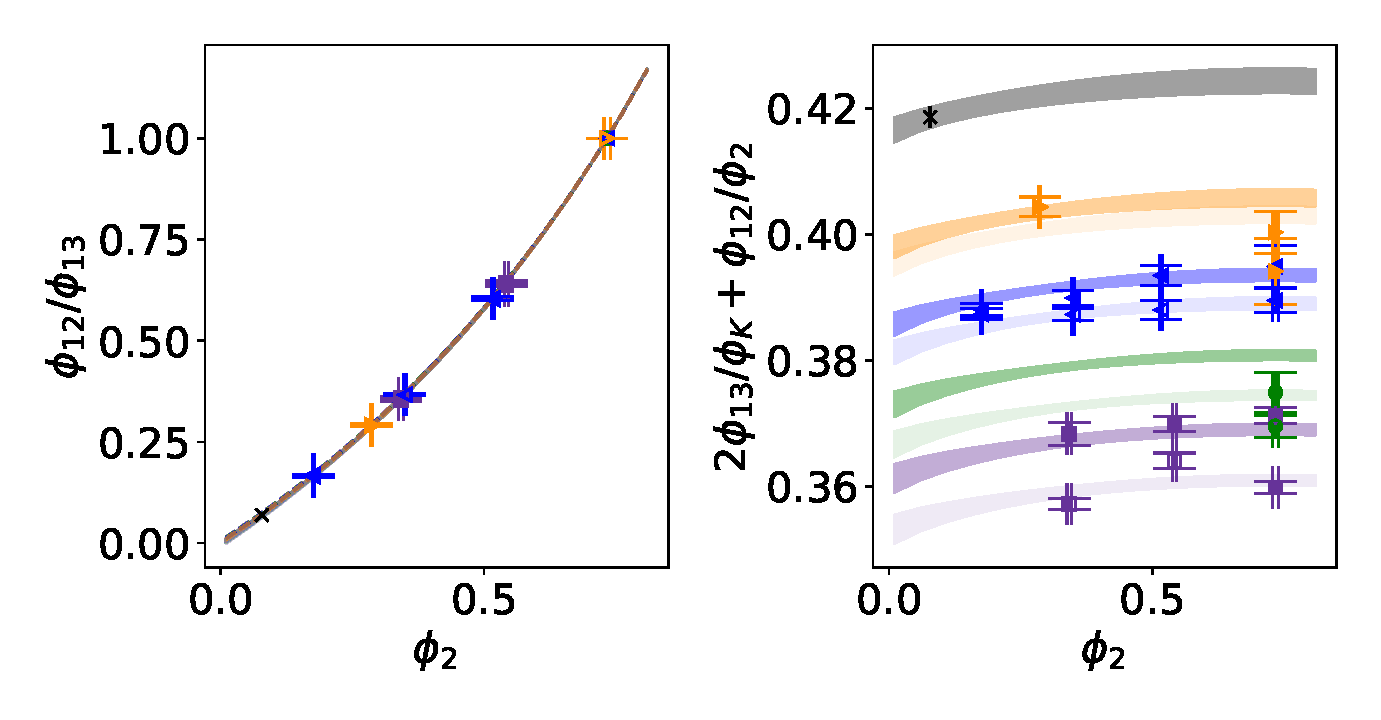
\includegraphics[scale=.5]{./apendices/figs_appex/mR_ratios_comb.pdf}
  	\caption{Chiral-continuum extrapolation fit to extract the quantities $\phi_{12,13}$ defined in eq.~(\ref{eq:phiij}) at the physical point and in the continuum. Empty point are obtained from our mixed action regularization, while filled points are obtained from the Wilson unitary setup. Purple squared symbols are $\beta=3.40$ ensembles, green circle symbols are $\beta=3.46$, blue left triangles are $\beta=3.55$ and orange right triangles are $\beta=3.70$. Only a subset of the available ensembles listed in Table \ref{apex_ensembles:tab:ens} are included in this preliminary analysis. The colored bands represent the mass-dependence for each lattice spacing: the darker bands corresponding to the Wilson unitary setup and the lighter ones to the mixed action setup. The gray band represents the continuum limit, and the black crossed point is the physical point result.} 
\label{fig:qm} 
\end{figure}


%%%%%%%%%%%%%%%%%%%%%%%%%%%%%%%%%%%%%%%%%%%%%%%%%%%%%%%%%%%
%%%%%%%%%%%%%%%%%%%%%%%%%%%%%%%%%%%%%%%%%%%%%%%%%%%%%%%%%%%
%%%%%%%%%%%%%%%%%%%%%%%%%%%%%%%%%%%%%%%%%%%%%%%%%%%%%%%%%%%
%%%%%%%%%%%%%%%%%%%%%%%%%%%%%%%%%%%%%%%%%%%%%%%%%%%%%%%%%%%

